\subsubsection{Administrationsbereich}
\label{sec:UmsetzungAdministrationsbereich}

Der entwickelte Prototyp stellt eine erste lauffähige Version einer Benutzeransicht dar. Der nächste Entwicklungsschritt ist die Implementierung des Administrationsbereiche und die Bereitstellung von APIs. Aufbauend auf gepflegten Ìnformationen im Administrationsbereich wird der Prototyp dann um dynamische Funktionalität erweitert. Das heißt die angezeigten Panoramas und die benachbarten Panoramas werden über eine API angefragt, die die Informationen aus der Datenbank lädt. Der Implementierungsprozess des Administrationsbereiches wird dabei sukzessiv anhand der vorgestellten Anwendungsfällen (siehe \nameref{sec:Adminstratoranwendungen} auf Seite \pageref{sec:Adminstratoranwendungen}) realisiert. Prioresiert werden dabei die Anwendungsfälle, die die Verwaltung der Panoramas, Infotexte und die Übersichtskarte betreffen (AFA05 bis AFA17).

Bevor mit der Implementierung begonnen werden kann wird noch ein einheitliches Design festgelegt, dass vor allem dem späteren Administrator das Verständnis erleichtert. Zu diesem einheitlichen Design Konzept zählt zum Beispiel das Farbschema von Buttons. So wurde beispielsweise festgelegt, dass ein roter Button immer das Löschen eines Datensatzes signalisiert und ein grüner immer das speichern eines Datensatzes. Darüber hinaus wurde entschieden die Gestaltung von Buttons, Informationsfenster und ähnlichem mit dem CSS\footnotemark\ Framework Bootstrap\footnotemark\ zu realisieren. Dadurch ist gewährleistet, dass alle Steuerungselemente in allen Browsern gleich aussehen und der Administrator Elemente durch ihr Aussehen wiedererkennen und darüber auf ihre Benutzung schließen kann. Durch diese Entscheidungen wird die Usability der Software erhöht und der Aufwand der zu erstellenden Dokumentation verringert.

\footnotetext{CSS steht für Cascading Style Sheets und beschreibt eine Skriptsprache, die dazu dient HTML-Elemente in Form und Farbe zu verändern.}

\footnotetext{Bootstrap ist ein open Source Projekt, in dem einheitlich das Design von verschiedenen HTML-Elemente definiert ist. Bootstrap ist ein Projekt des Internetkonzerns Twitter und ist besonders dafür geeignet ein einheitliches Look and Feel einer Webseite in allen Browsern zu erzeugen.}

Aufbauend auf Administratoranwendungsfällen und Designkonzept werden Tickets erstellt, deren Inhalt die Implementierung der Infotext- und Fotoverwaltung ist. Zur Verdeutlichung der eingesetzten Technologien und des Entwicklunsablaufs wird im Folgenden eine stark vereinfachte Fotoverwaltungsseite implementiert. Implementiert werden soll eine Seite, die alle Fotos der Datenbank mit Namen und Beschreibung anzeigt. Zustätzlich soll es dem Administrator möglich sein auf den Namen eines Fotos zu klicken, woraufhin ihm weitere Informationen angezeigt werden.

Zur Implementierung dieses Szenarios wird zunächst ein HTML-Dokument angefertigt, dass das Grundgerüst der Fotoverwaltung darstellt. In diesem Grundgerüst könnten bestimmte Elemente, wie zum Beispiel die Navigationsbar am oberen Rand (vergleiche \abbildung{MockupBackend}) der Seite oder der Titel der Seite, statisch codiert werden. Zur Vereinfachung soll aber nur der Titel der Seite gesetzt werden und eine Überschrift. Das folgende \listing{HTML_Anwendungsbeispiel} zeigt das angefertigte HTML-Dokument.

\lstinputlisting[language=HTML,caption={statisches HTML},label={lst:HTML_Anwendungsbeispiel}]{Listings/HTML_Anwendungsbeispiel.html}

Im Anschluss daran muss die Seite um dynamisch generierten Inhalt erweitert werden. Dynamischer Inhalt ist im gegeben Anwendungsfall das Anzeigen aller Fotos, die bereits in der Datenbank sind. Um dieses Verhalten zu realisieren muss eine Anfrage an die Datenbank gestellt werden und danach muss für jeden Eintrag in der Datenbank HTML Quellcode geschrieben werden. Das nachfolgende \listing{HTML mit PHP} zeigt die Implementierung mit PHP.

\lstinputlisting[language=HTML,caption={Dynamisches schreiben von HTML mit PHP},label={lst:HTML mit PHP}]{Listings/HTML_mit_PHP.php}

Zu sehen ist die Anfrage an die Datenbank, die durch die PHP-Funktion "`mysql\_query"' (Zeile 5) realisiert wird, das Durchlaufen jeden Datenbanksatzes in einer Schleife (Zeile 6ff.) und das schreiben von HTML mit dem PHP "`echo"'-Befehl.

Zum Abschluss wird das klicken auf den Fotonamen implementiert. Diese Benutzerinteraktion kann am besten auf dem Clientsystem des Benutzers (Internetbrowser) mit Javascript verarbeitet werden, da keine weiteren Informationen vom Server benötigt werden und zusätzliche Anfragen so vermieden werden. Javascript-Routinen werden meistens als Funktionen formuliert, die aufgerufen werden, wenn ein bestimmtes Ereignis eintritt. Im \listing{HTML mit PHP} ist ein solcher Funktionsaufruf in Zeile 9 zu sehen. Die Funktion "`toggleDescription"' wird aufgerufen sobald auf das <p>-Tag geklickt wird. Als Parameter wird dieser Funktion das eigene HTML-Element, also das <p>-Tag, mitgegeben. Die Javascript-Funktion ist in \listing{Javascript Snippet} dargestellt.

\lstinputlisting[language=JavaScript,caption={Auf Benutzerinteraktion reagieren mit Javascript},label={lst:Javascript Snippet}]{Listings/Javascript_Snippet.js}

Alle dargestellten Listings könnten dabei in einem Dokument stehen, das vom dem Administrator über seinen Internetbrowser angefragt wird.
Wie bereits erwähnt ist diese Darstellung der Implementierung sehr stark vereinfacht. Die Quelldateien, die die Fotoverwaltung im vorliegenden Projekt implementieren, sind zu umfangreich, um sie an dieser Stelle zu präsentieren. Die implementierte Fotoverwaltung wird in folgendem Bildschirmfoto zur Veranschaulichung dargestellt:

%TODO: Bildschirmfoto ohne Pixelfehler machen.
\begin{figure}[htb]
\centering
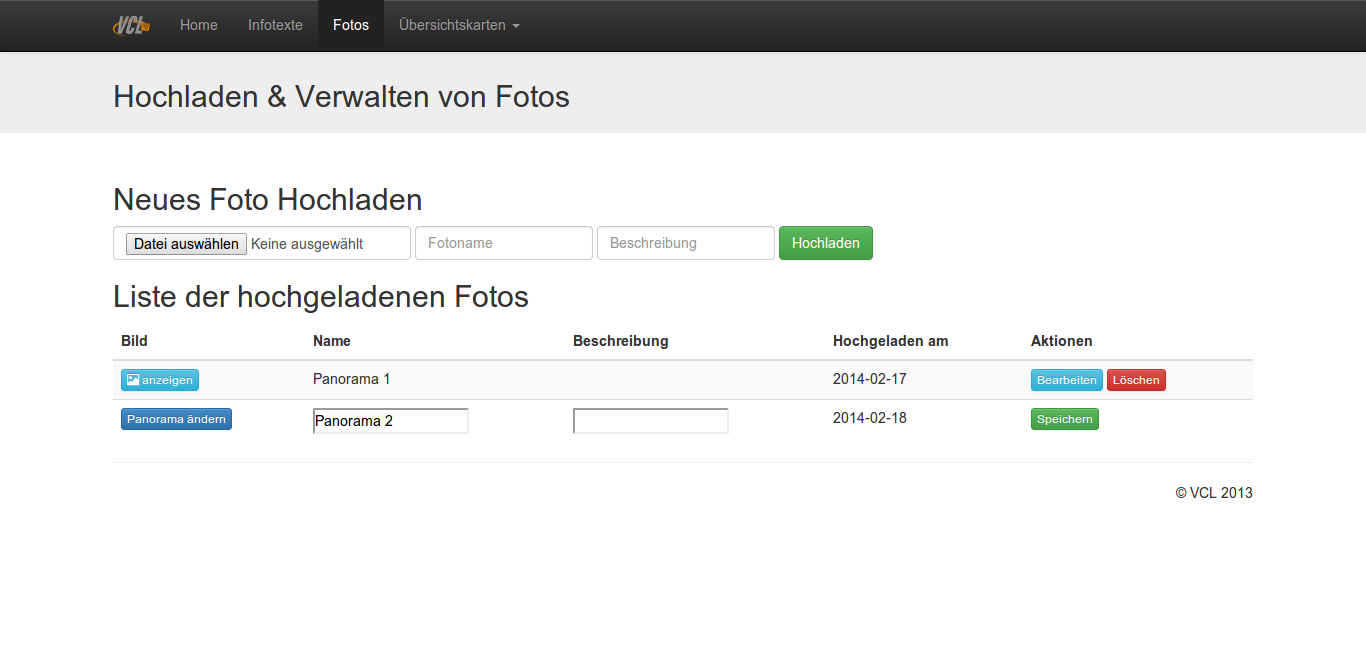
\includegraphics[width=1.0\textwidth]{Fotoverwaltung.png}
\caption[Fotoverwaltung]{Bildschirmfoto der implementierten Fotoverwaltung}
\label{fig:Fotoverwaltung}
\end{figure}

In einem solchen Entwicklungszyklus wurde auch die Verwaltung der Infotexte und die Übersichtskarte implementiert. Bildschirmfotos dieser Bereiche sind im Anhang dargstellt.